Task 3 explores the option of using a Variational Autoencoder (VAE). In order to train our first model, we will use the MNIST dataset \cite{deng2012mnist} containing 60,000 training samples as well as 10,000 test samples of handwritten numbers and normalise the pixel values between 0 and 1. The task specifies what the model should look like: 

\begin{itemize}
    \item two-dimensional latent space
    \item multivariate diagonal Gaussian distribution as approximate posterior $q_\phi(z \vert x)$
    \item Encoder (outputs the mean and standard deviation of $q_\phi(z \vert x)$): 
    \begin{itemize}
        \item 2 hidden layers with 256 units each and ReLU activation functions
        \item multivariate diagonal Gaussian distribution as likelihood $p_\theta(x \vert z)$
    \end{itemize}
    \item Decoder (outputs only the mean of $p_\theta(x \vert z)$):
    \begin{itemize}
        \item 2 hidden layers with 256 units each and ReLU activation functions
        \item standard deviation for the decoder distribution as one floating-point, trainable variable
    \end{itemize}
    \item multivariate diagonal standard normal distribution as the prior $p(z)$
\end{itemize}

Additionally, the Adam optimiser is used with a learning rate of 0.001, as well as a batch size of 128 for training. The libraries used in our code are depicted in table \ref{tab:vae-libraries} together with the functionalities that we utilised.  \\

\begin{table}[hbt!]
\centering
%\resizebox{\textwidth}{!}
{%
\begin{tabular}{|l|l|}
\hline
Tensorflow \cite{tensorflow2015-whitepaper}  & \begin{tabular}[c]{@{}l@{}}download the MNIST dataset\\ \& implement Early Stopping\end{tabular}  \\ \hline
Numpy \cite{harris2020array}    &    generate random samples  from a normal (Gaussian) distribution    \\ \hline
Matplotlib \cite{Hunter:2007} & visualise the constructed and generated images \\ \hline
\end{tabular}%
}
\caption{Libraries and their utilised functions for the task of VAE}
\label{tab:vae-libraries}
\end{table}


\textbf{1. What activation functions should be used for the mean and standard deviation of the approximate posterior and the likelihood and why?} \\

The choice of activation functions for the mean and standard deviation in a VAE is critical due to the properties of Gaussian distributions. For the mean \(\mu\) of the approximate posterior \(q_\phi(z | x)\), a linear activation function is appropriate as the mean can take on any real value. Hence, no activation function, or the identity function, is typically used:

\begin{equation}
\mu = W_{\mu}h + b_{\mu}
\end{equation}

where \(W_{\mu}\) and \(b_{\mu}\) are the weights and biases for the mean, and \(h\) is the output from the last hidden layer of the encoder.

For the standard deviation \(\sigma\), we require an activation function that ensures the output is positive, as the standard deviation must be non-negative. The softplus function is commonly used for this purpose:

\begin{equation}
\sigma = \log(1 + \exp(W_{\sigma}h + b_{\sigma}))
\end{equation}

where \(W_{\sigma}\) and \(b_{\sigma}\) are the weights and biases for the standard deviation.

The softplus function is smooth and gradually increases, avoiding any abrupt changes in the gradient, which benefits the stability of the learning process. Additionally, it closely approximates a ReLU function for large input values, effectively preventing the standard deviation from collapsing to zero.

For the likelihood \(p_\theta(x | z)\), the decoder outputs only the mean, and since the pixel values are normalized between 0 and 1, a sigmoid activation function is used to ensure the output is within this range:

\begin{equation}
\hat{x} = \sigma(W_{\hat{x}}z + b_{\hat{x}})
\end{equation}

where \(\sigma(\cdot)\) is the sigmoid function, ensuring that the reconstructed input \(\hat{x}\) is in the range \([0, 1]\), corresponding to the normalized pixel values.\\


\textbf{2. What might be the reason if we obtain good reconstructed but bad generated digits?} \\

There exist multiple possible reasons for the VAE to produce badly generated digits like learning rate, training duration, or loss function. However, it is apparent that the latent space of our model is very small. This can result in the model not having enough capacity to represent the diversity of the data during generation. Because of this, we will increase the latent space in part 5 of this task. \\

% Train the VAE (training set) and do the following experiments (test set) after the 1st epoch, the 5th epoch, the 25th epoch, the 50th epoch, and after the optimisation converged:
\textbf{3. Train the VAE} \\

In question 3, we train the VAE. After the 1st, 5th, 25th, and 50th epoch, we will plot the latent representation, plot reconstructed digits, and plot generated digits. Additionally, we do the same after convergence. To determine when the optimisation converges, we make use of Early Stopping which monitors \texttt{val\_loss} and uses patience of 5. The exact point of convergence will differ since the VAE does not work deterministically. In the figures we provided in the report, Early Stopping happened after epoch 55. \\

\textbf{3.1. Plot the latent representation} \\

We have our results of transformation of the latent space of a Variational Autoencoder (VAE) as it is trained over multiple epochs. The plots show the latent representations of a test dataset, where each point corresponds to a high-dimensional data instance compressed into two latent dimensions for visualization purposes. The color indicates class labels, which are not used during the unsupervised training of the VAE but are shown here to demonstrate the clustering capability of the model.

Subplot \ref{fig:latentRep1} depicts the latent space after 1 epoch of training. The data points are largely overlapped, indicating that the VAE has not yet learned to separate the different classes effectively in the latent space.

Subplot \ref{fig:latentRep5} shows the latent space after 5 epochs. The beginnings of cluster formation can be observed, with the VAE starting to distinguish between classes, although considerable overlap still exists.

Subplot \ref{fig:latentRep25} represents the latent space after 25 epochs. The clusters are more defined, showing that the VAE has improved in mapping similar data points (from the same class) closer together in the latent space while separating different classes.

Subplot \ref{fig:latentRep50} presents the latent space after 50 epochs. The clusters are well-defined and mostly non-overlapping, illustrating that the VAE is now capable of organizing the data in a way that similar instances are located in proximity to each other, forming distinct clusters corresponding to the different classes. This suggests a matured learning where the encoder part of the VAE has developed a more structured understanding of the data.
% explanation for latent representation

\begin{figure}[H]
    \centering
    \begin{subfigure}[b]{0.45\textwidth}
        \centering
        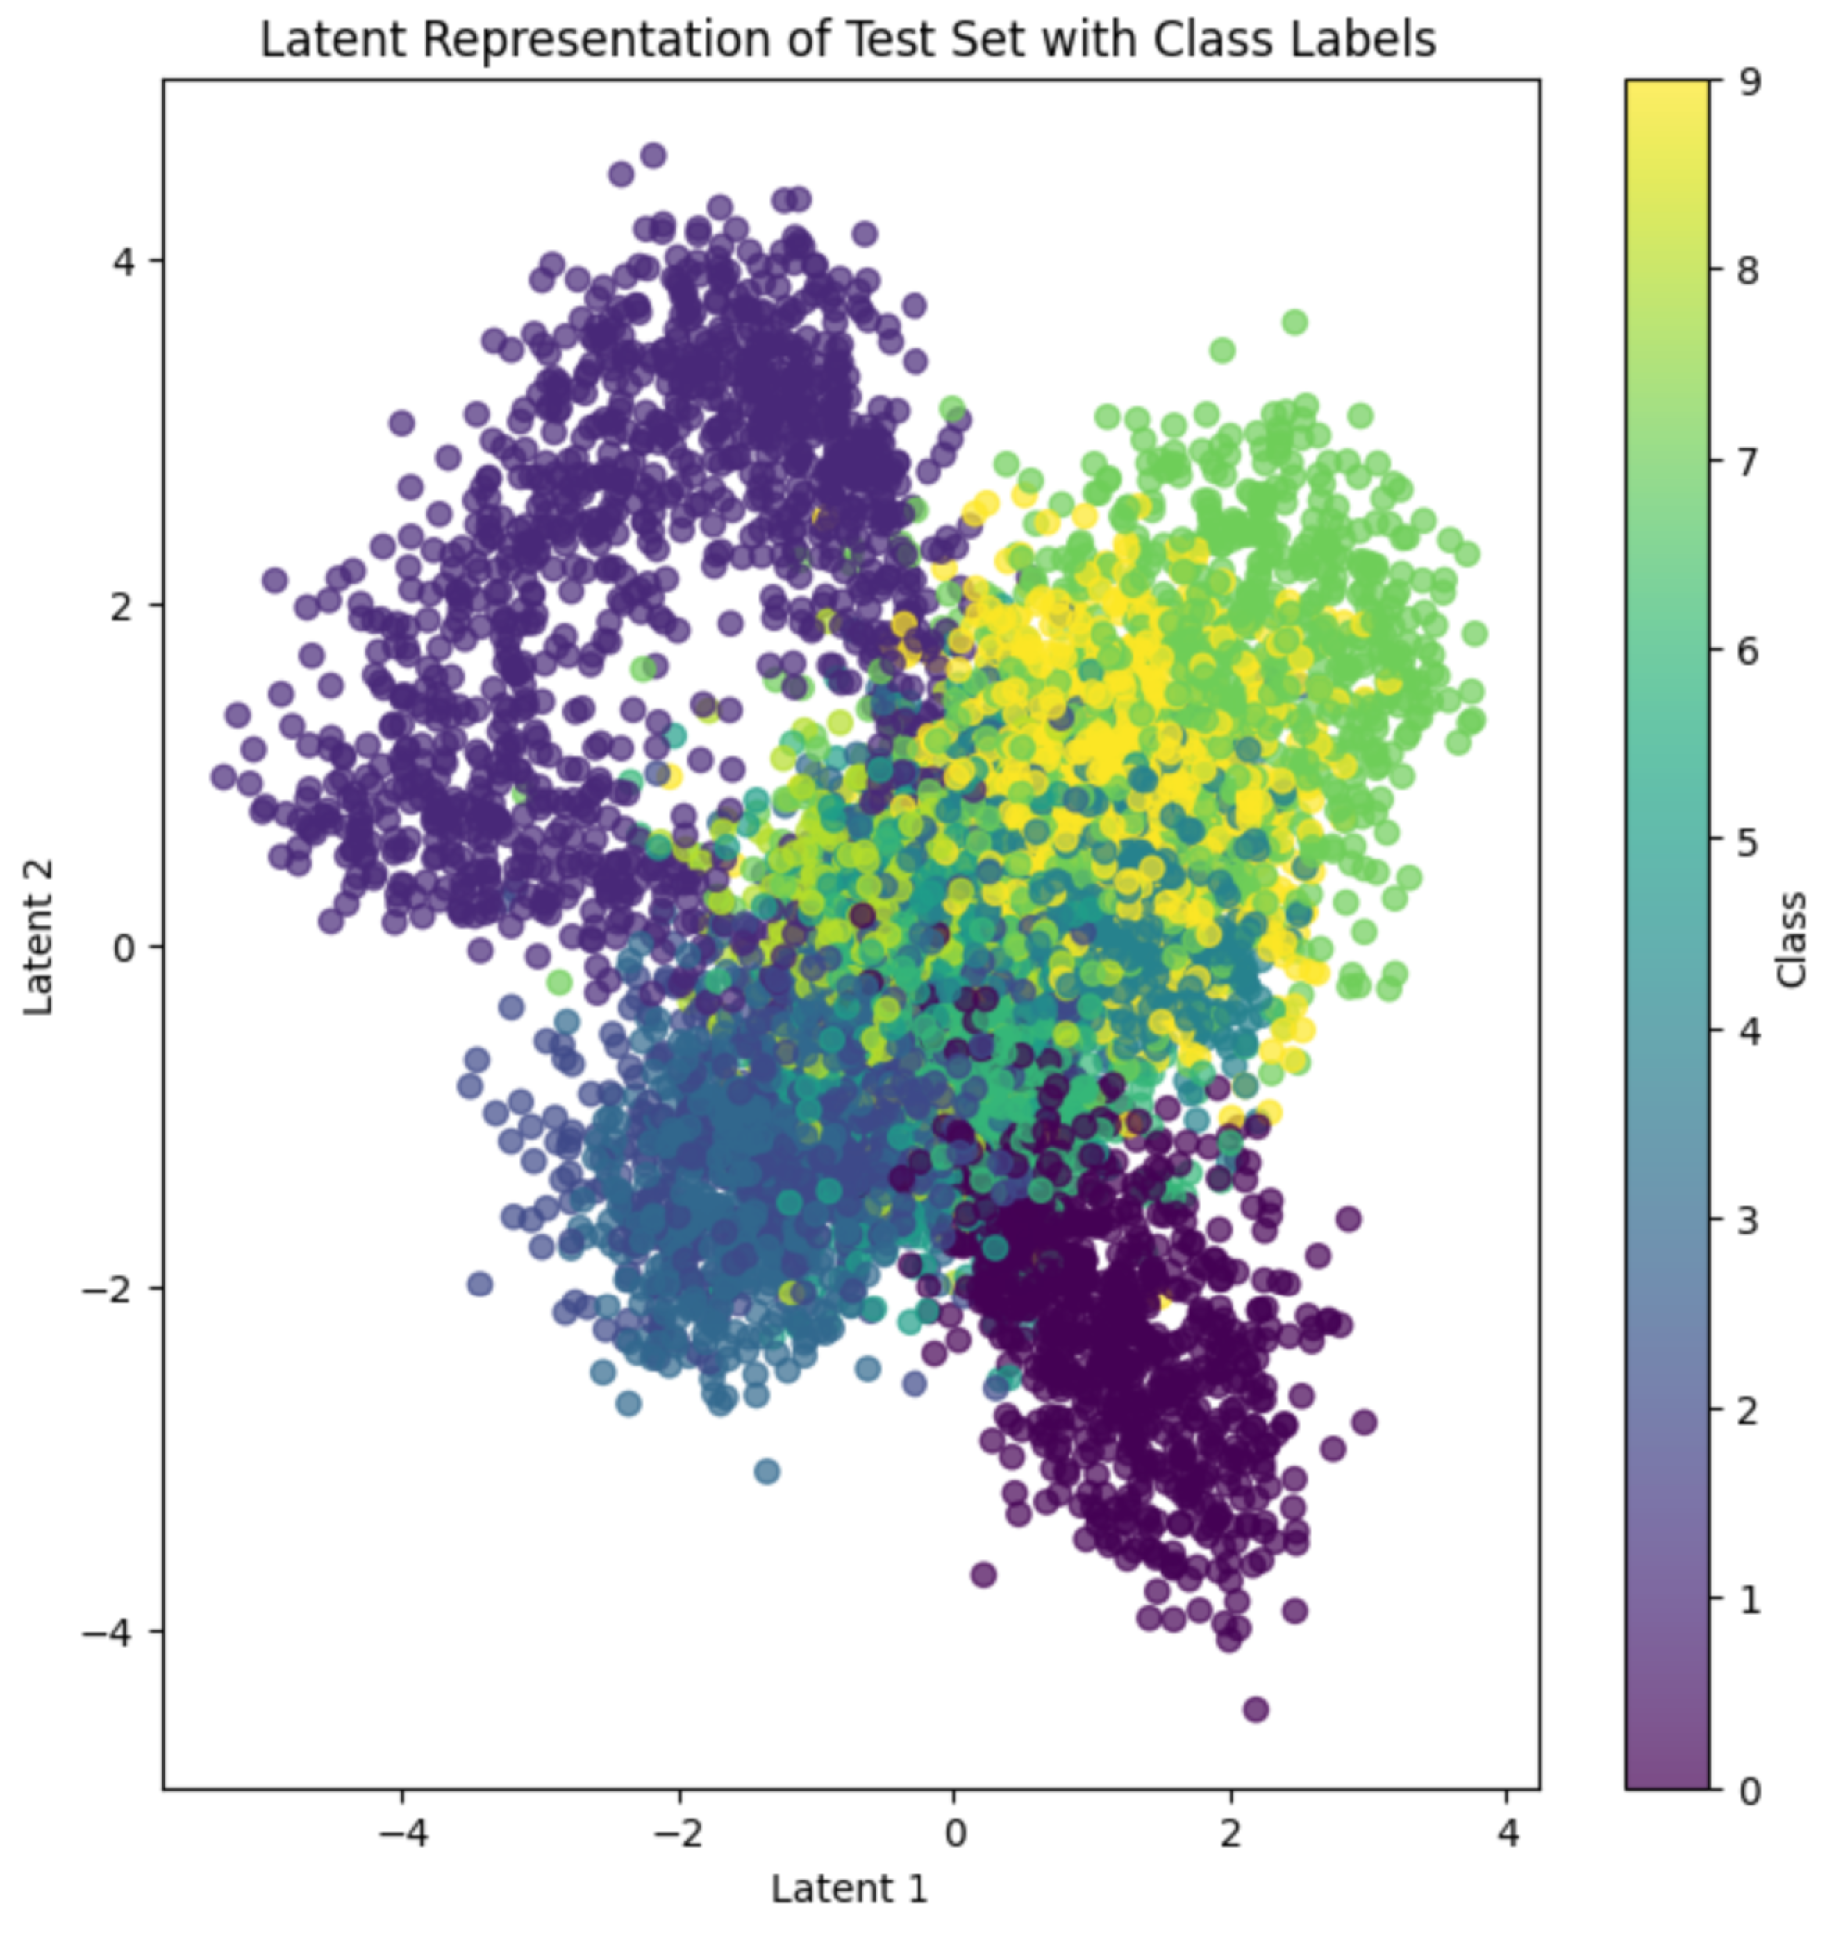
\includegraphics[width=\textwidth]{images/3-latentRep1.png}
        \caption{1 epoch}
        \label{fig:latentRep1}
    \end{subfigure}
    \begin{subfigure}[b]{0.45\textwidth}
        \centering
        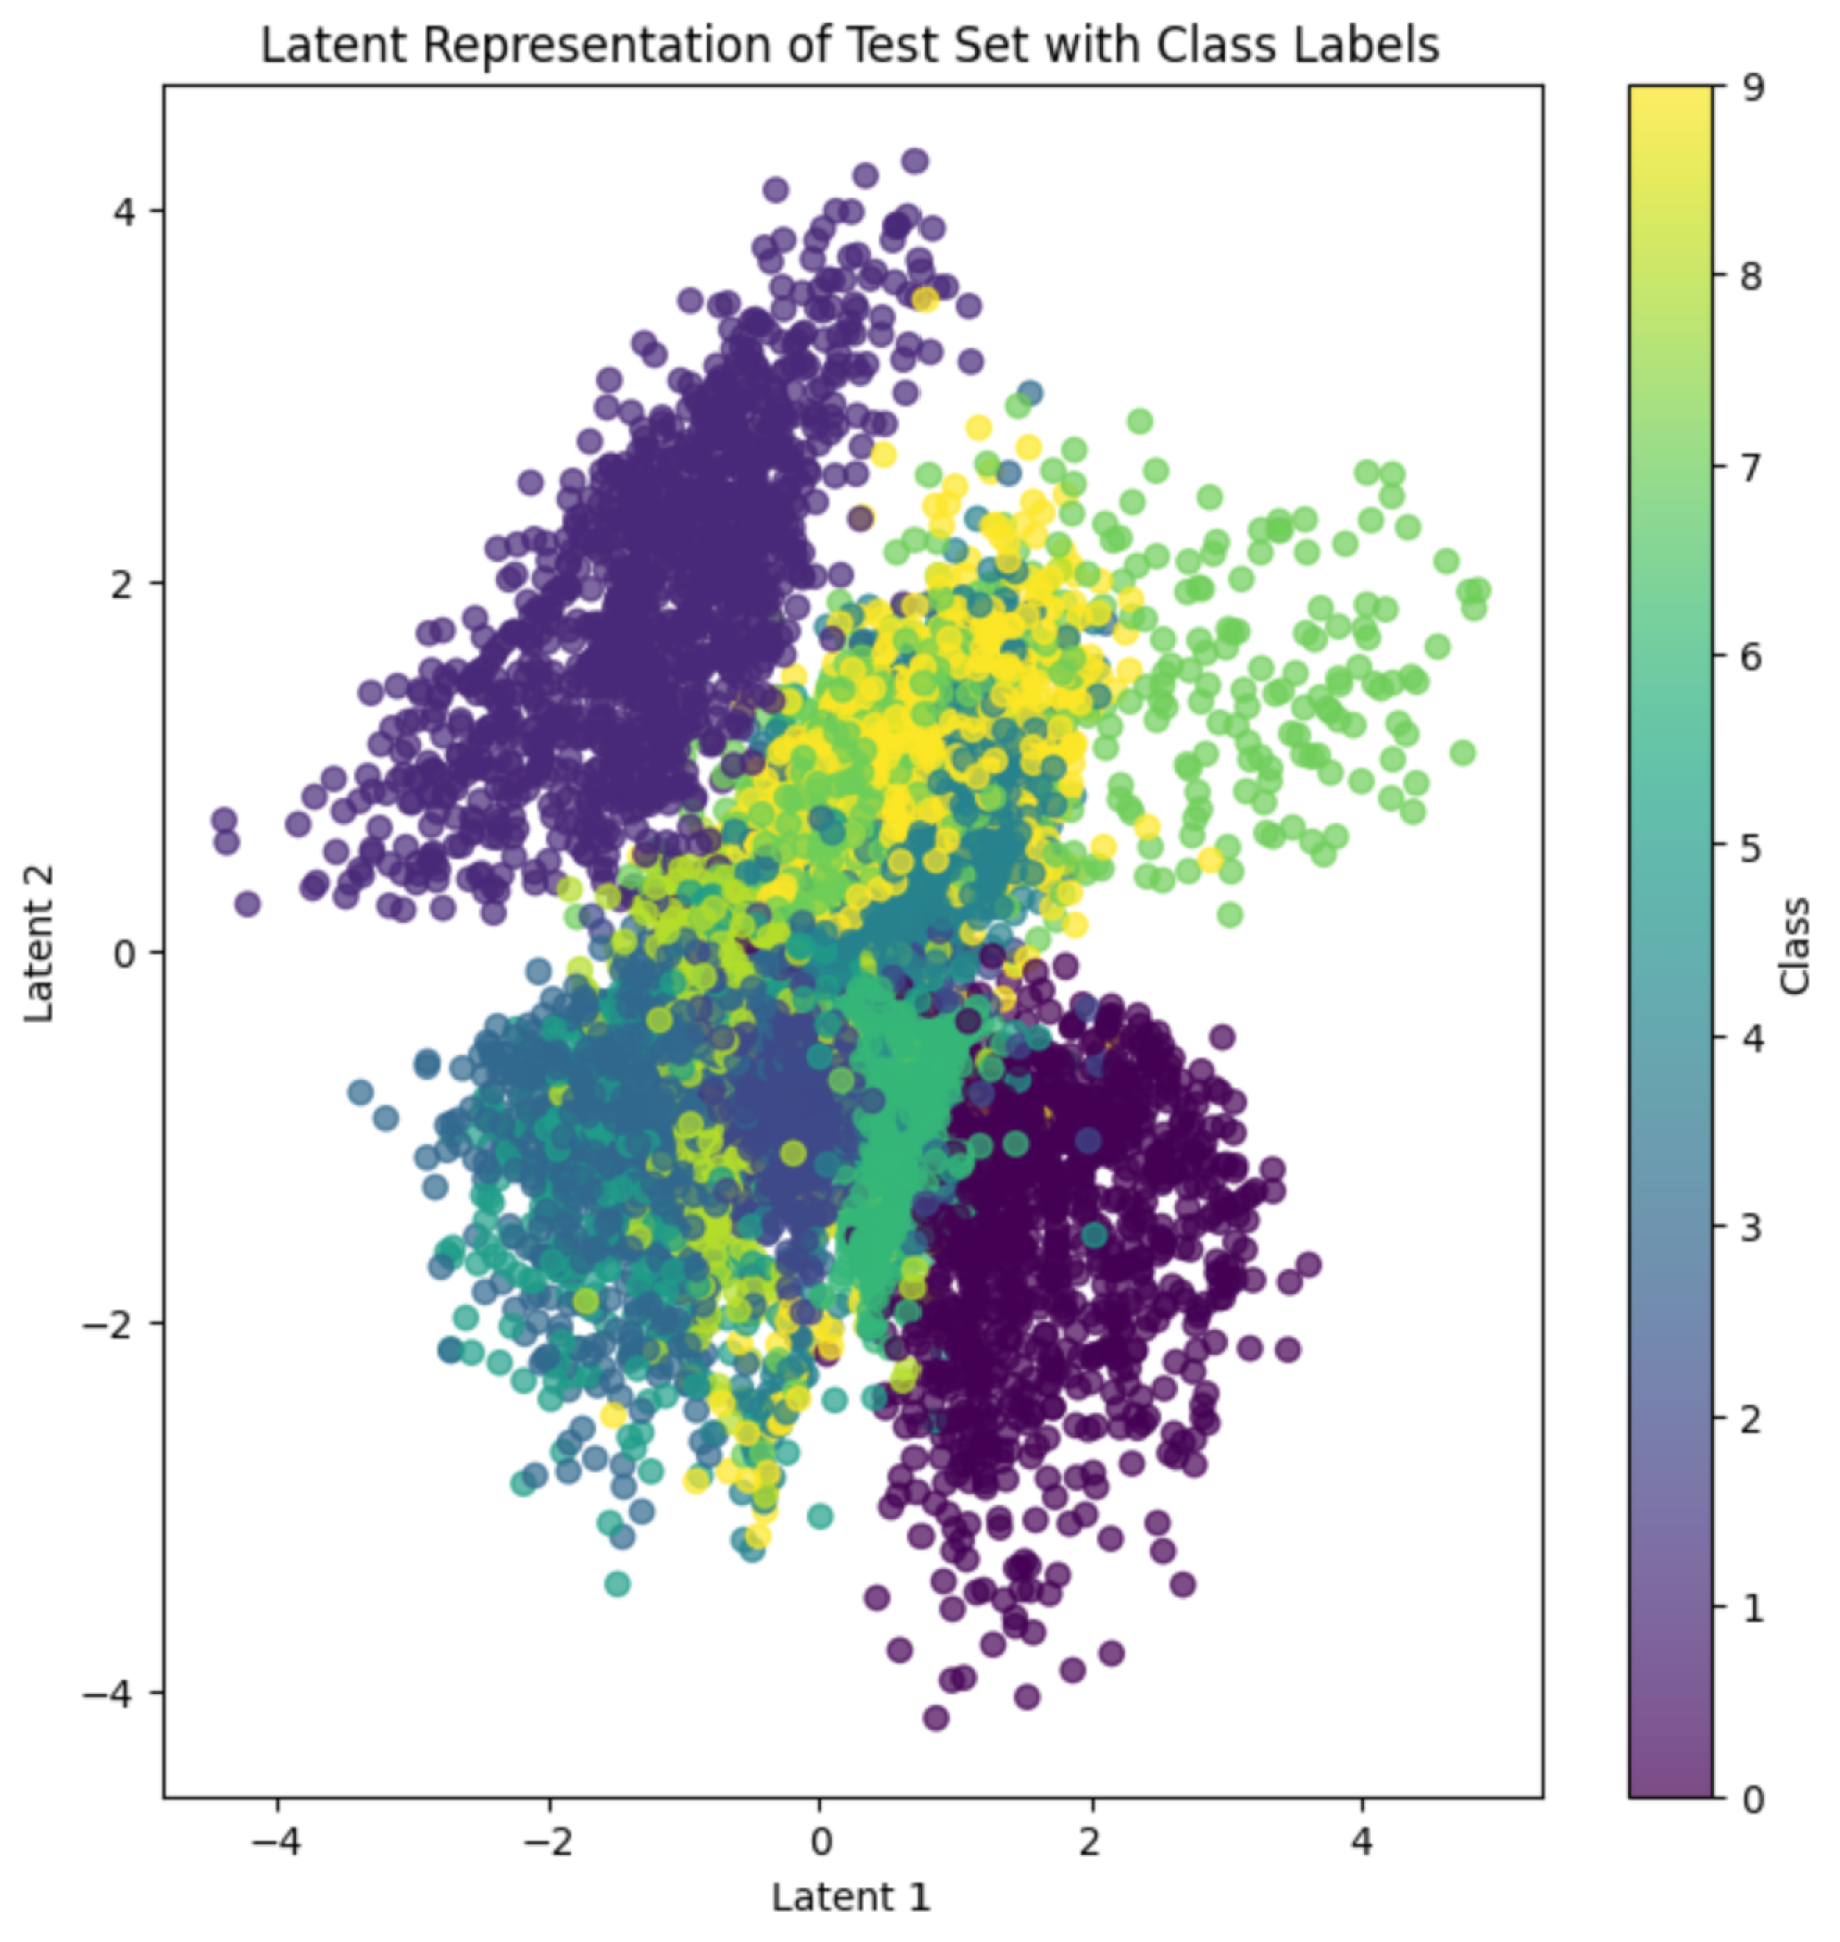
\includegraphics[width=\textwidth]{images/3-latentRep5.png}
        \caption{5 epochs}
        \label{fig:latentRep5}
    \end{subfigure}
    \begin{subfigure}[b]{0.45\textwidth}
        \centering
        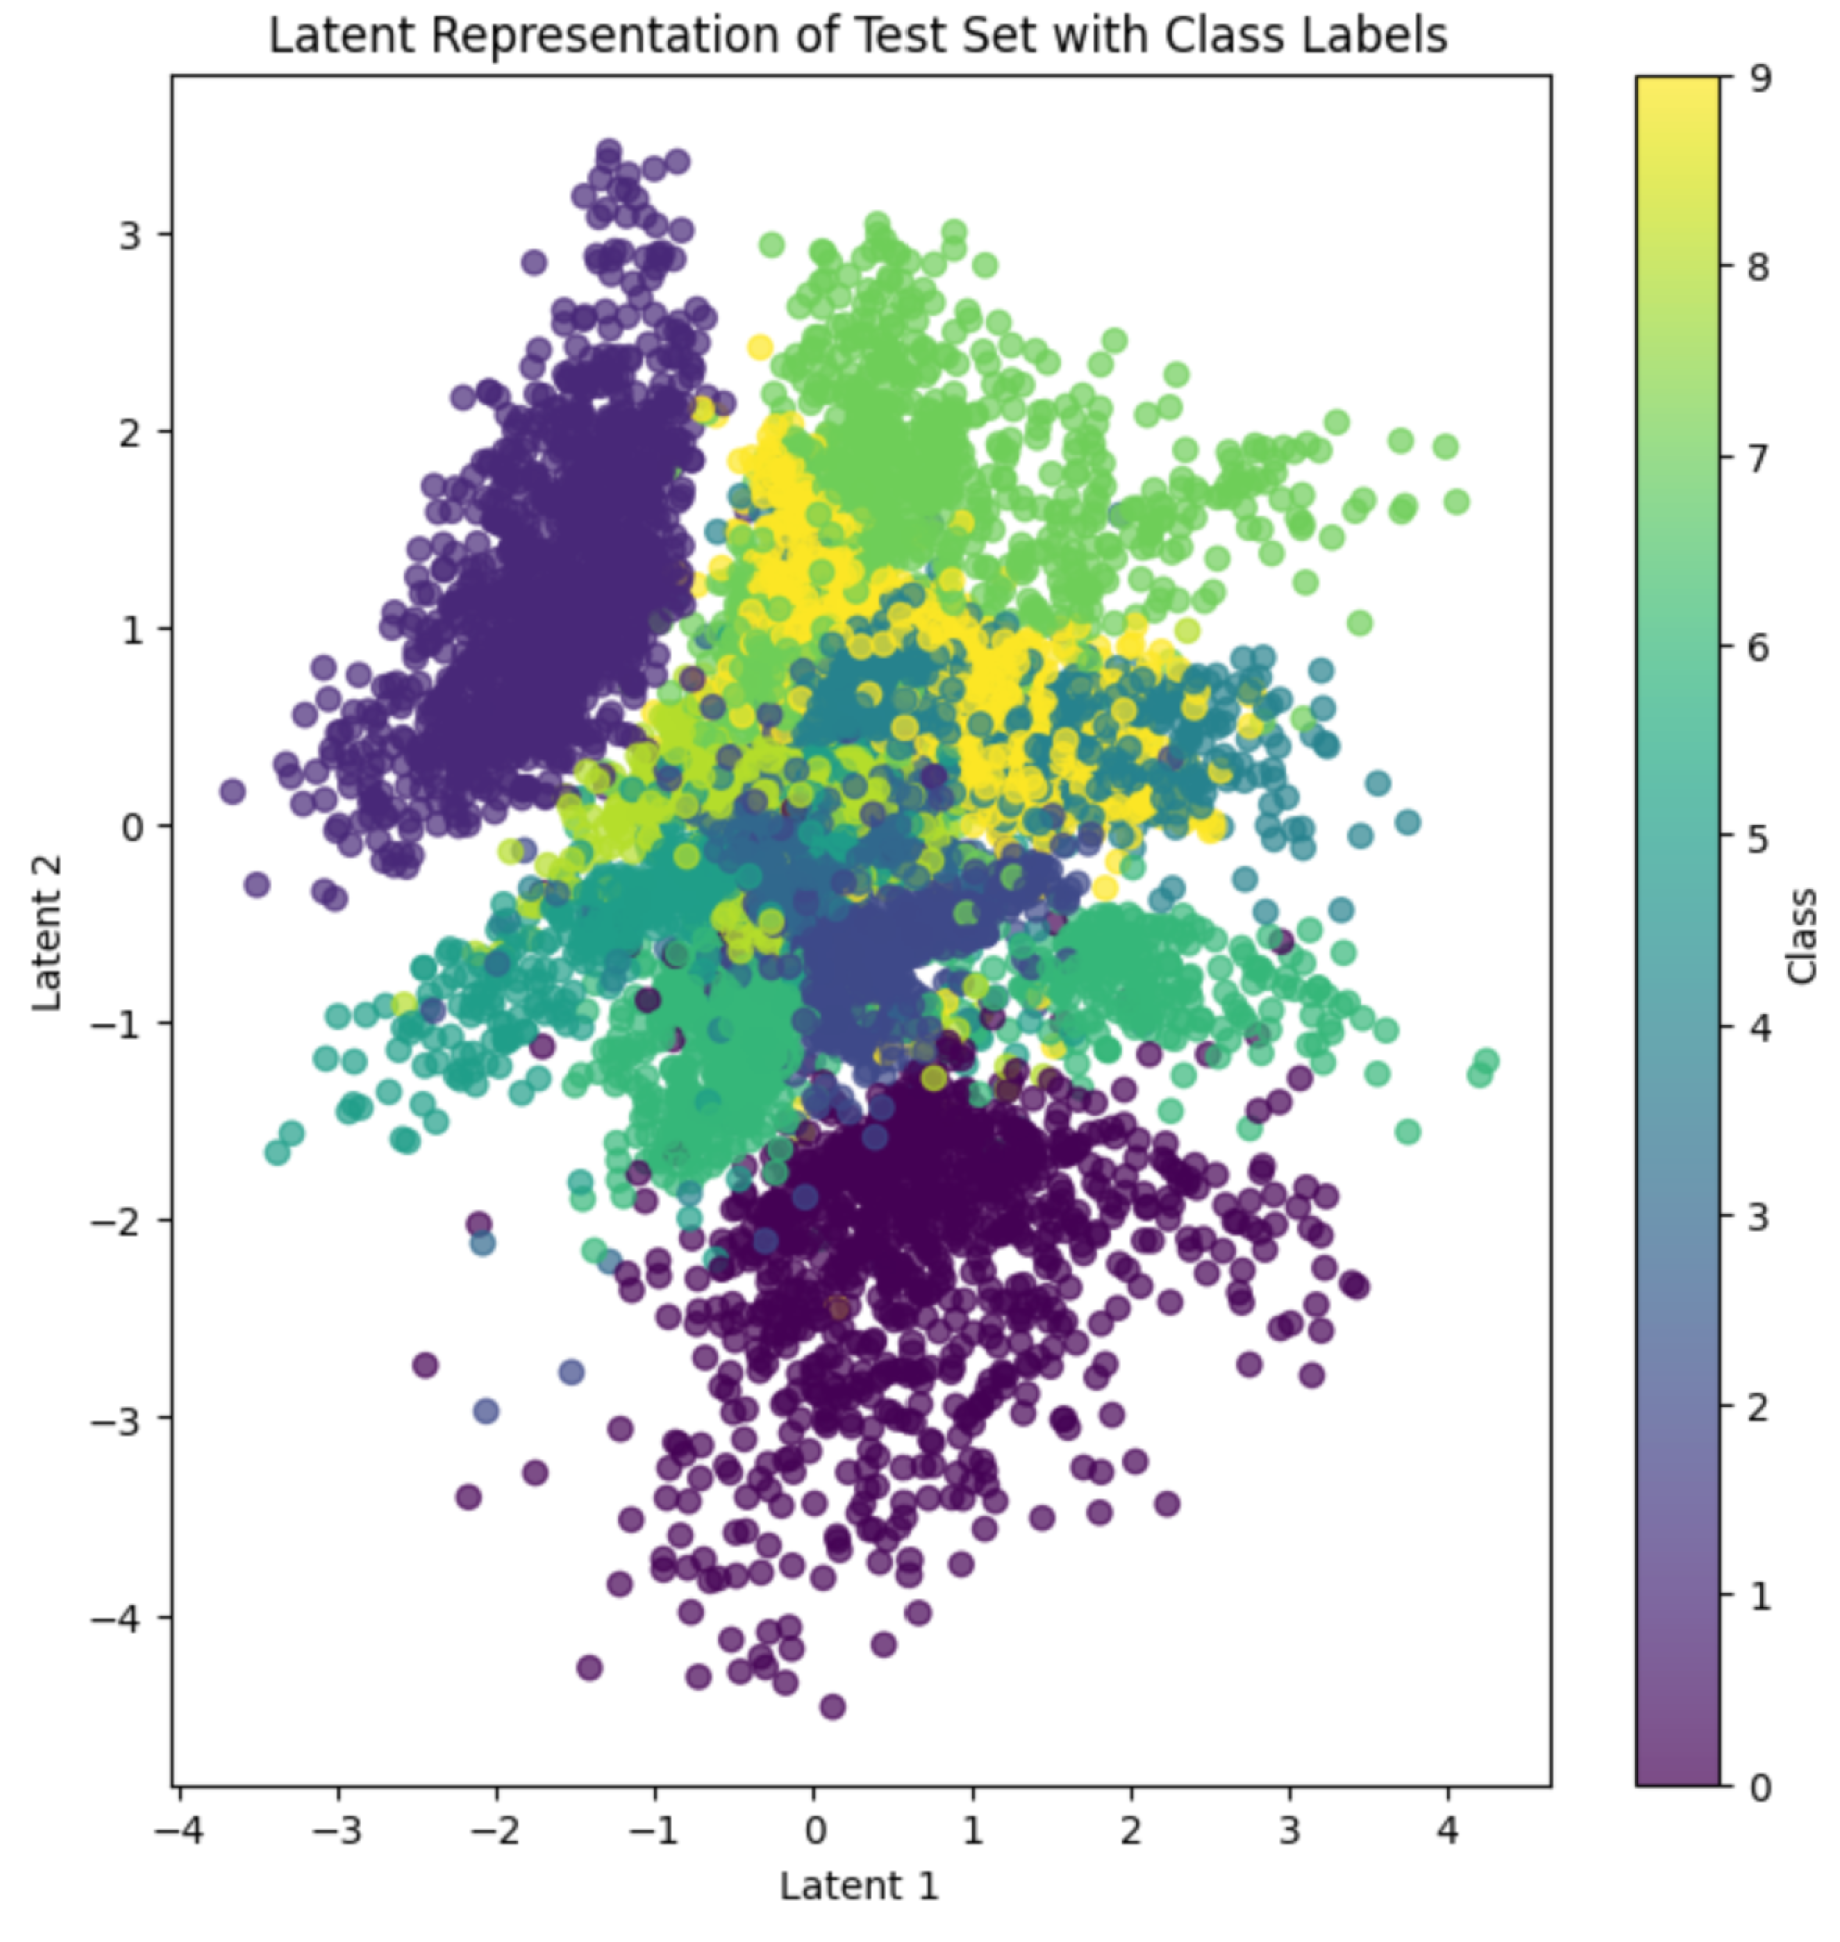
\includegraphics[width=\textwidth]{images/3-latentRep25.png}
        \caption{25 epochs}
        \label{fig:latentRep25}
    \end{subfigure}
    \begin{subfigure}[b]{0.45\textwidth}
        \centering
        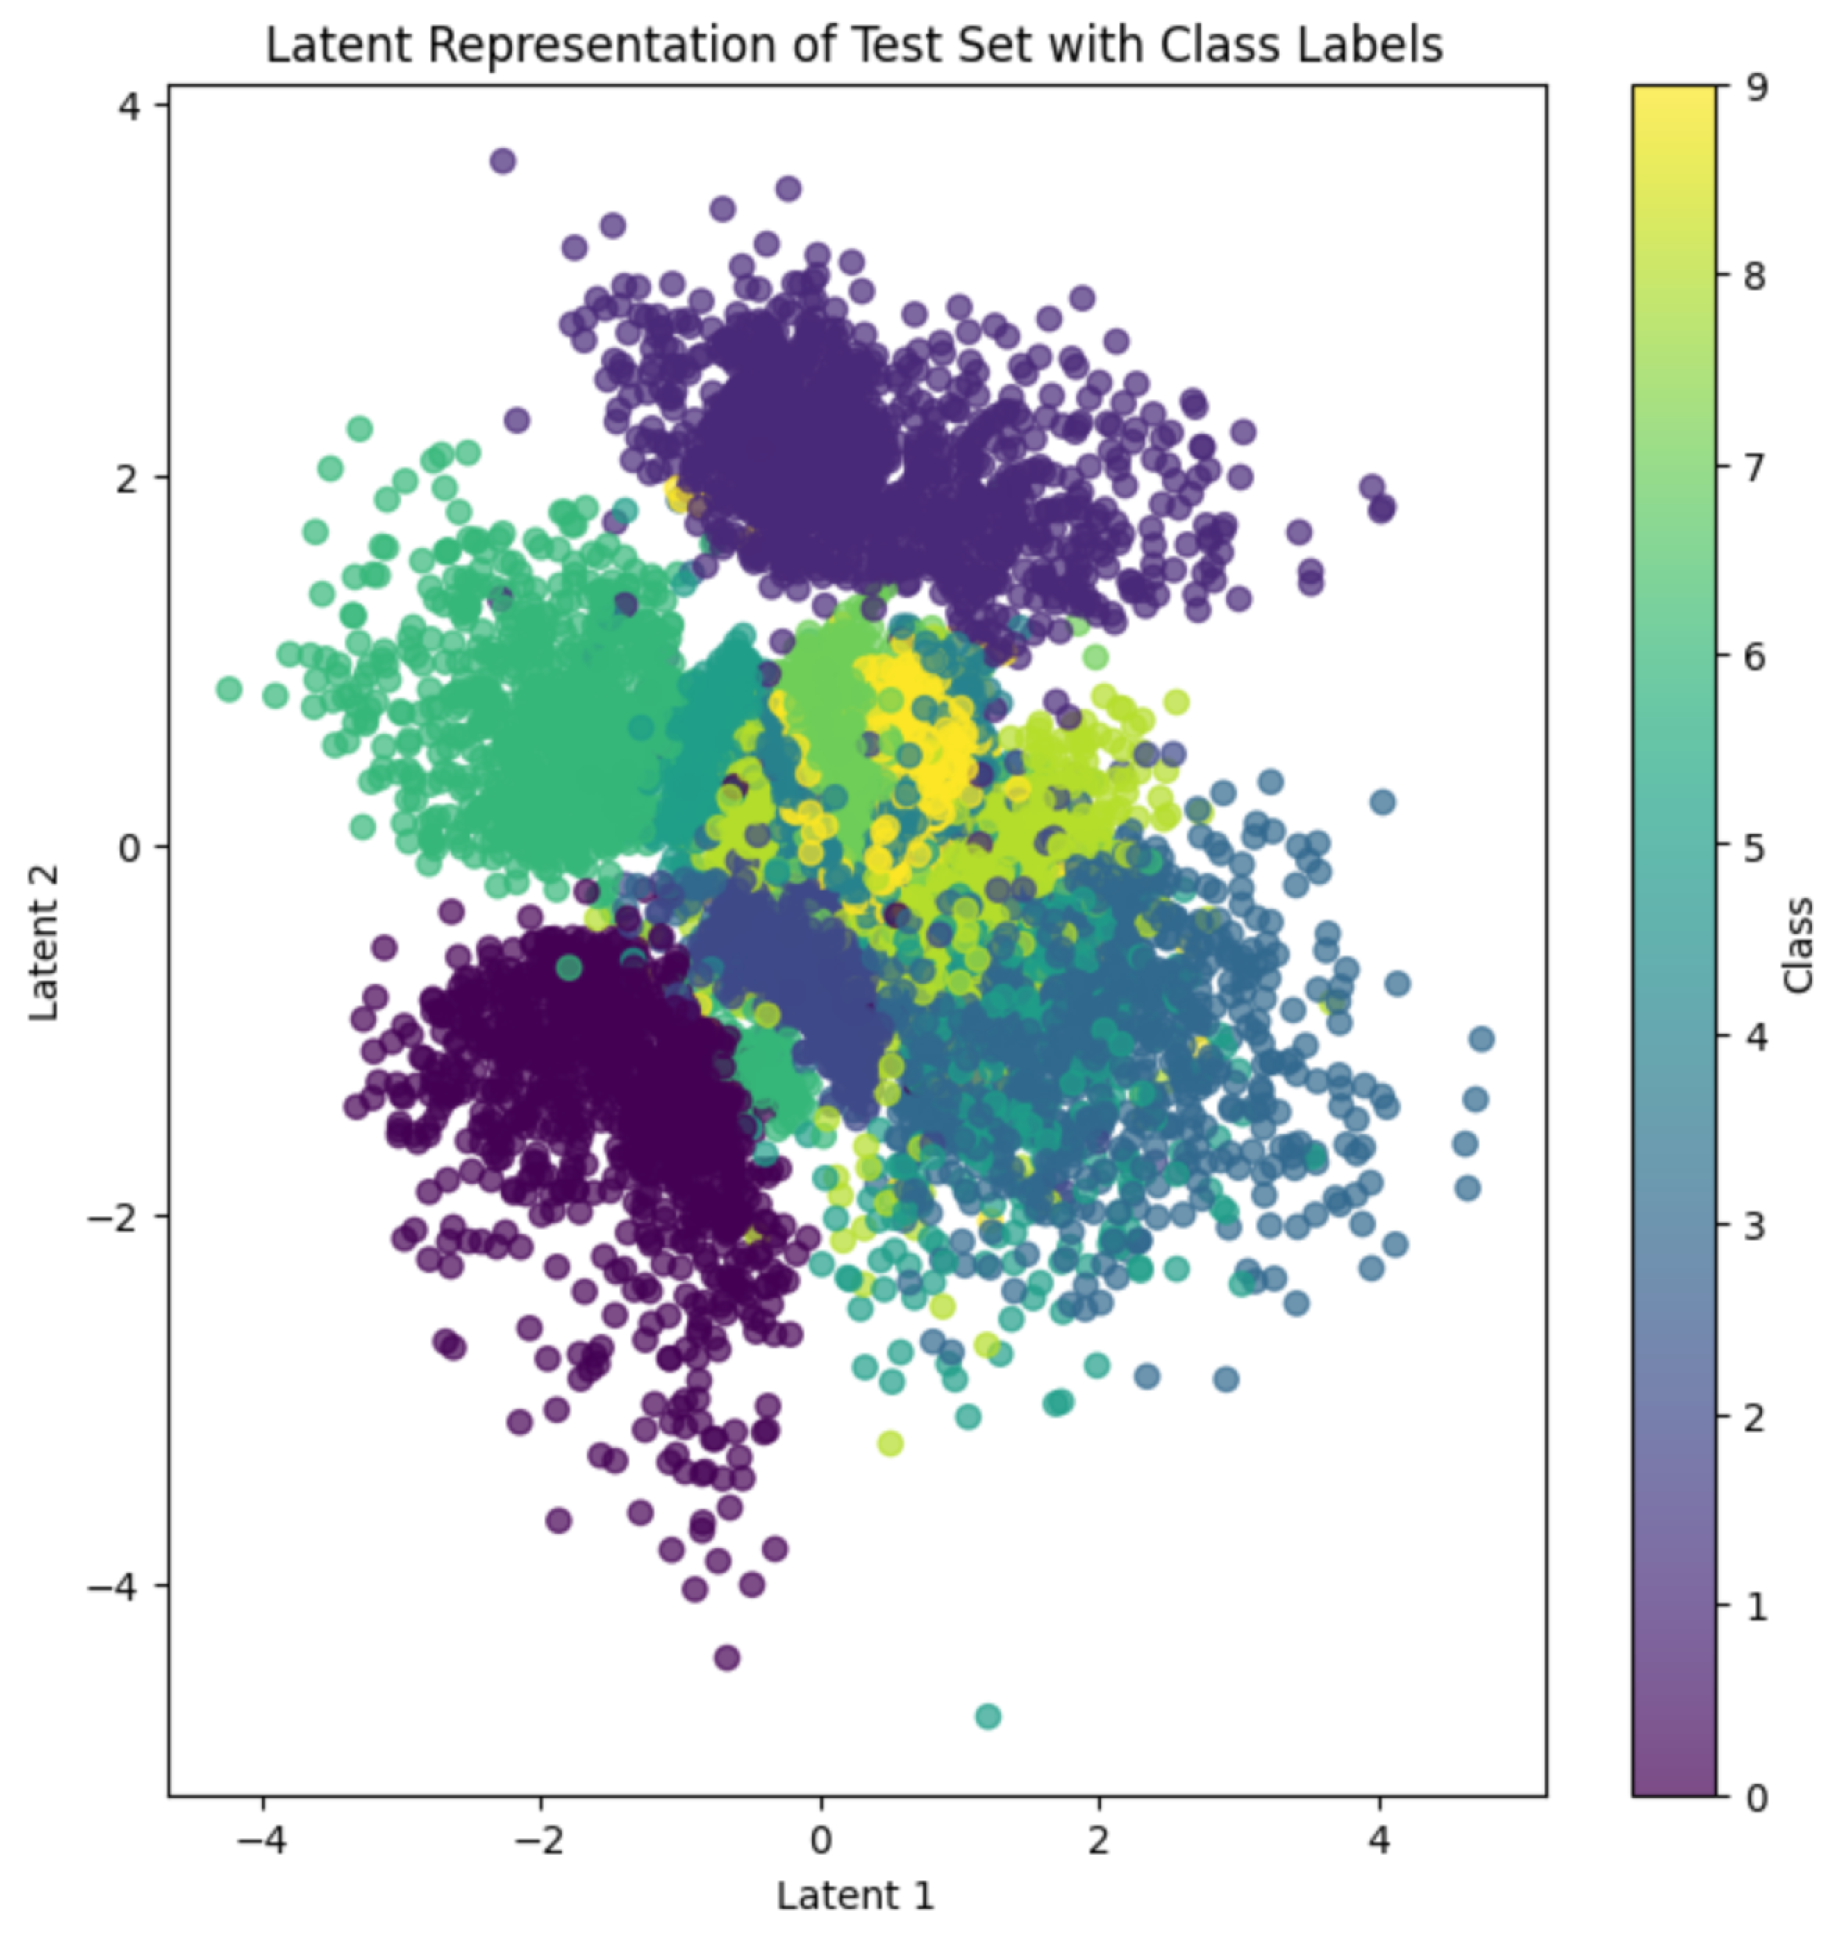
\includegraphics[width=\textwidth]{images/3-latentRep50.png}
        \caption{50 epochs}
        \label{fig:latentRep50}
    \end{subfigure}
    % latent representation after optimisation converged
    \caption{Latent Representation after different numbers of epochs}
    \label{fig:latentRep}
\end{figure}

\begin{figure}[H]\ContinuedFloat
    \centering
    \begin{subfigure}[b]{0.45\textwidth}
        \centering
        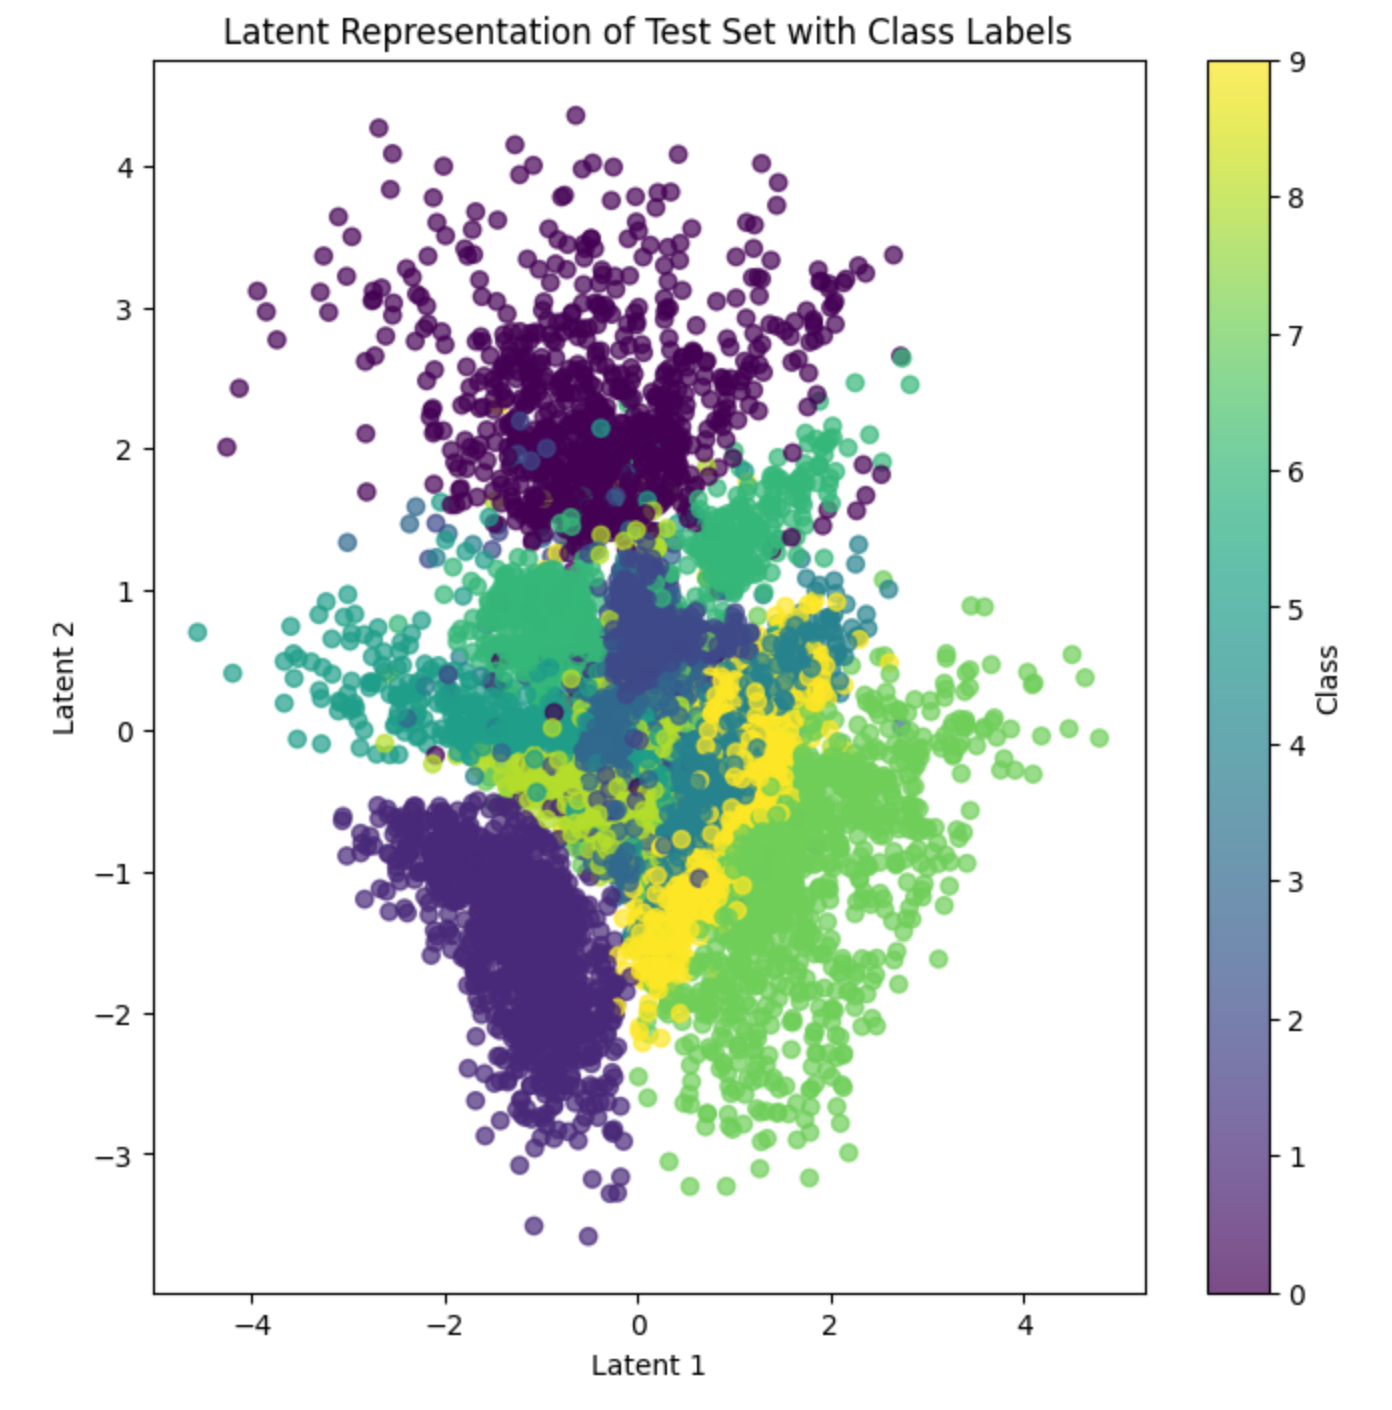
\includegraphics[width=\textwidth]{images/3-latentRepCon.png}
        \caption{after convergence}
        \label{fig:latentRepCon}
    \end{subfigure}
    \caption{Latent Representation after different numbers of epochs}
    \label{fig:latentRep2}
\end{figure}

\textbf{3.2. Plot 15 reconstructed digits and the corresponding original ones.} \\

To generate the reconstructed digits, we use \texttt{$vae.predict(x\_test)$}. Plotting them creates figure \ref{fig:reconstructed}, the subfigures show different training times. After only 1 (\ref{fig:reconstructed1}) and 5 (\ref{fig:reconstructed5}) epochs, it is difficult to achieve proper results for all digits. Increasing the training time to 25 (\ref{fig:reconstructed25}) or 50 (\ref{fig:reconstructed50}) epochs helps to recognize most of the digits and only shows a small difference between both training times. 

Overall, the model works well and 12 of the reconstructed digits depict the correct number for 25 and 50 epochs. Two out of the three errors result from the same digits: A 4 turns into a 9. This mistake is easy to retrace. The two lines on top of the 4 just need to be connected with a slight arc to change the number accordingly. The third error recreates a 4 for 25 epochs, even though the original digit was a 5. This mistake seems unnecessary since multiple lines do not align. For 50 epochs the same digit is problematic and shows a 0. An explanation for the mistakes on this digit is the sloppy handwriting which is distinctly different to a properly written 5. After convergence, even this digit is correctly displayed in the reconstruction. All of the reconstructed digits display a blurriness to them which is to be expected. However, there are methods to reduce blurriness, which again include a larger latent space. \\ 

\begin{figure}[H]
    \centering
    \begin{subfigure}[b]{\textwidth}
        \centering
        
\includegraphics[width=\textwidth]{images/3-originalR.png}
        \caption{Original digits}
        \label{fig:originalR}
    \end{subfigure}
    \begin{subfigure}[b]{\textwidth}
        \centering
        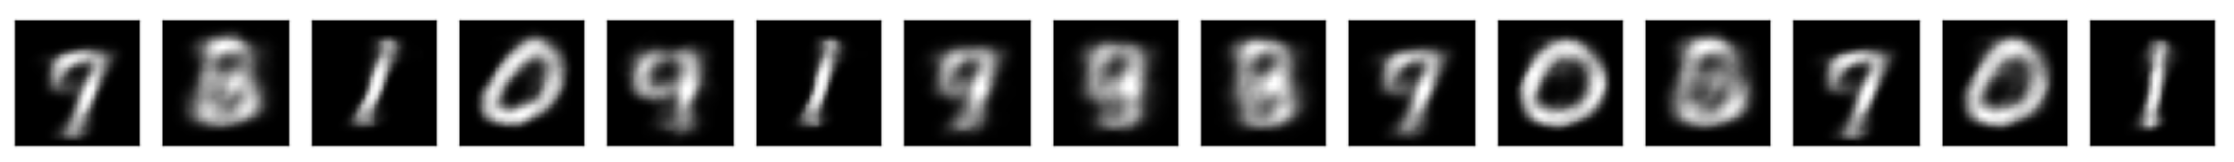
\includegraphics[width=\textwidth]{images/3-reconstructed1.png}
        \caption{1 epoch}
        \label{fig:reconstructed1}
    \end{subfigure}
    \begin{subfigure}[b]{\textwidth}
        \centering
        
\includegraphics[width=\textwidth]{images/3-reconstructed5.png}
        \caption{5 epochs}
        \label{fig:reconstructed5}
    \end{subfigure}
    \begin{subfigure}[b]{\textwidth}
        \centering
        
\includegraphics[width=\textwidth]{images/3-reconstructed25.png}
        \caption{25 epochs}
        \label{fig:reconstructed25}
    \end{subfigure}
    \begin{subfigure}[b]{\textwidth}
        \centering
        
\includegraphics[width=\textwidth]{images/3-reconstructed50.png}
        \caption{50 epochs}
        \label{fig:reconstructed50}
    \end{subfigure}
    \begin{subfigure}[b]{\textwidth}
        \centering
        
\includegraphics[width=\textwidth]{images/3-reconstructedCon.png}
        \caption{after convergence}
        \label{fig:reconstructedCon}
    \end{subfigure}
    \caption{Reconstructed digits after different numbers of epochs}
    \label{fig:reconstructed}
\end{figure}

\textbf{3.3. Plot 15 generated digits, i.e., decode 15 samples from the prior.} \\

To generate new digits, we use \texttt{$decoder.predict(random\_samples)$}. Plotting them creates figure \ref{fig:generated}, the subfigures show different training times. After 1 epoch (\ref{fig:generated1}), barely any digits can be recognized. This changes for 5 (\ref{fig:generated5}) and 25 epochs (\ref{fig:generated25}).  For 50 epochs (\ref{fig:generated50}) the identifiability decreases again slightly. 

Most of the generated digits in figure \ref{fig:generated25} can be recognized as a specific number. The first generated digit could be interpreted either as 1 or as 7. Since the original images showing the number 1 however only consist of a line, the first generated digit most likely corresponds to the number 7. The second digit shows the number 8 with the left side less pigmented making it similar to the number 3. The third digit depicts a problem we already encountered in the reconstructed digits: Numbers 4 and 9 look similar. Both 4 and 9 could be interpreted with a preference towards the number 9. The second digit in the second row is the only image that cannot certainly be assigned a specific number. The remaining digits are easy to recognize and assign. \\

\begin{figure}[H]
    \centering
    \begin{subfigure}[b]{\textwidth}
        \centering
        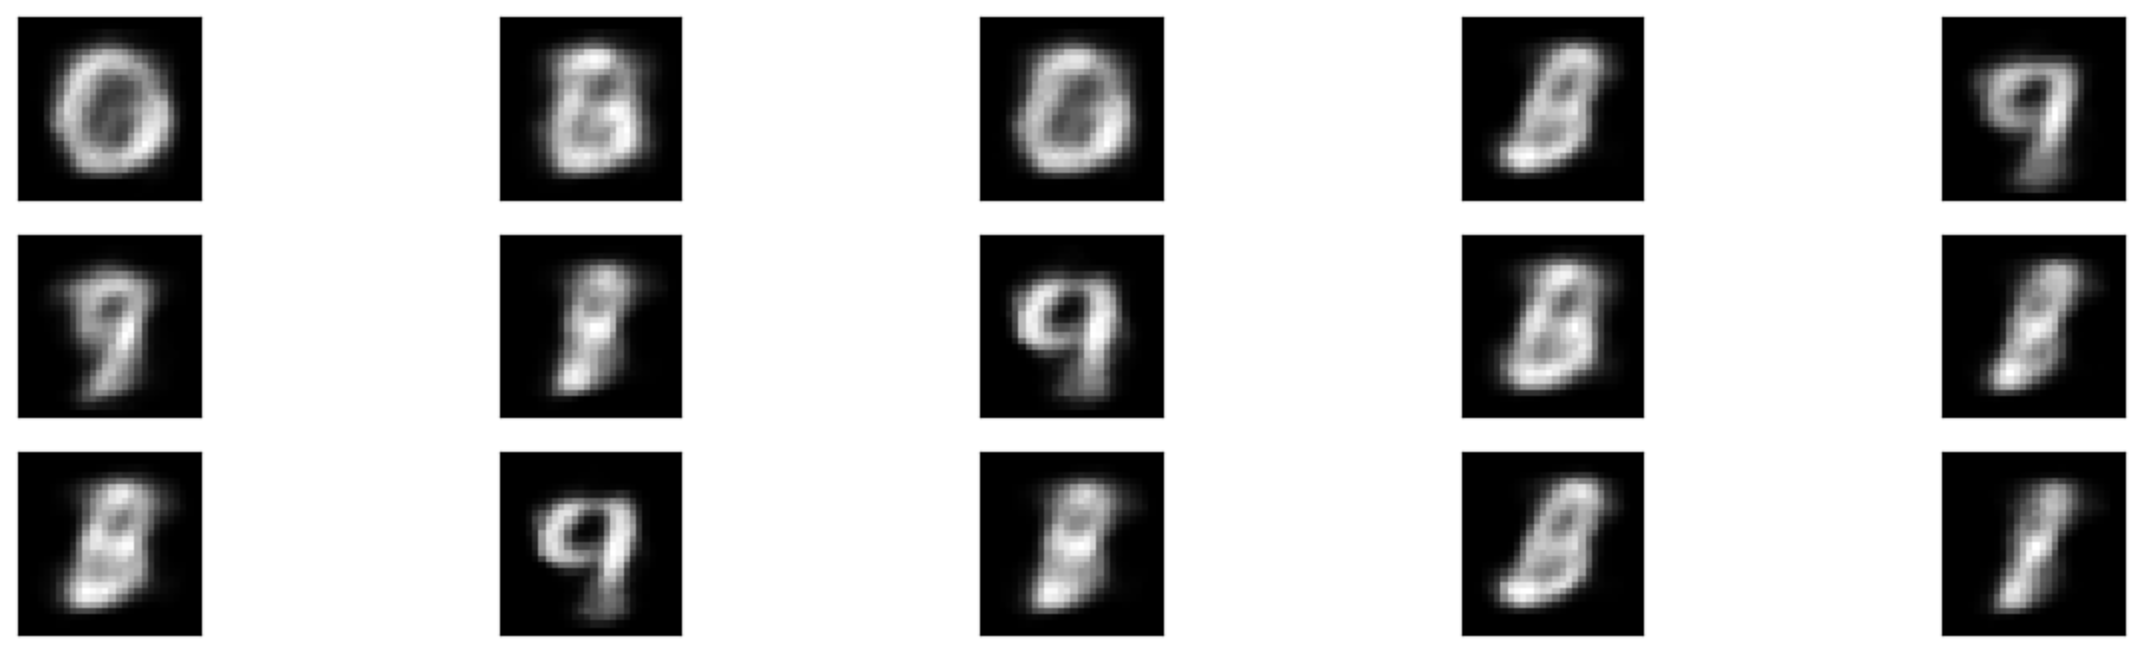
\includegraphics[width=\textwidth]{images/3-generated1.png}
        \caption{1 epoch}
        \label{fig:generated1}
    \end{subfigure}
    \begin{subfigure}[b]{\textwidth}
        \centering
        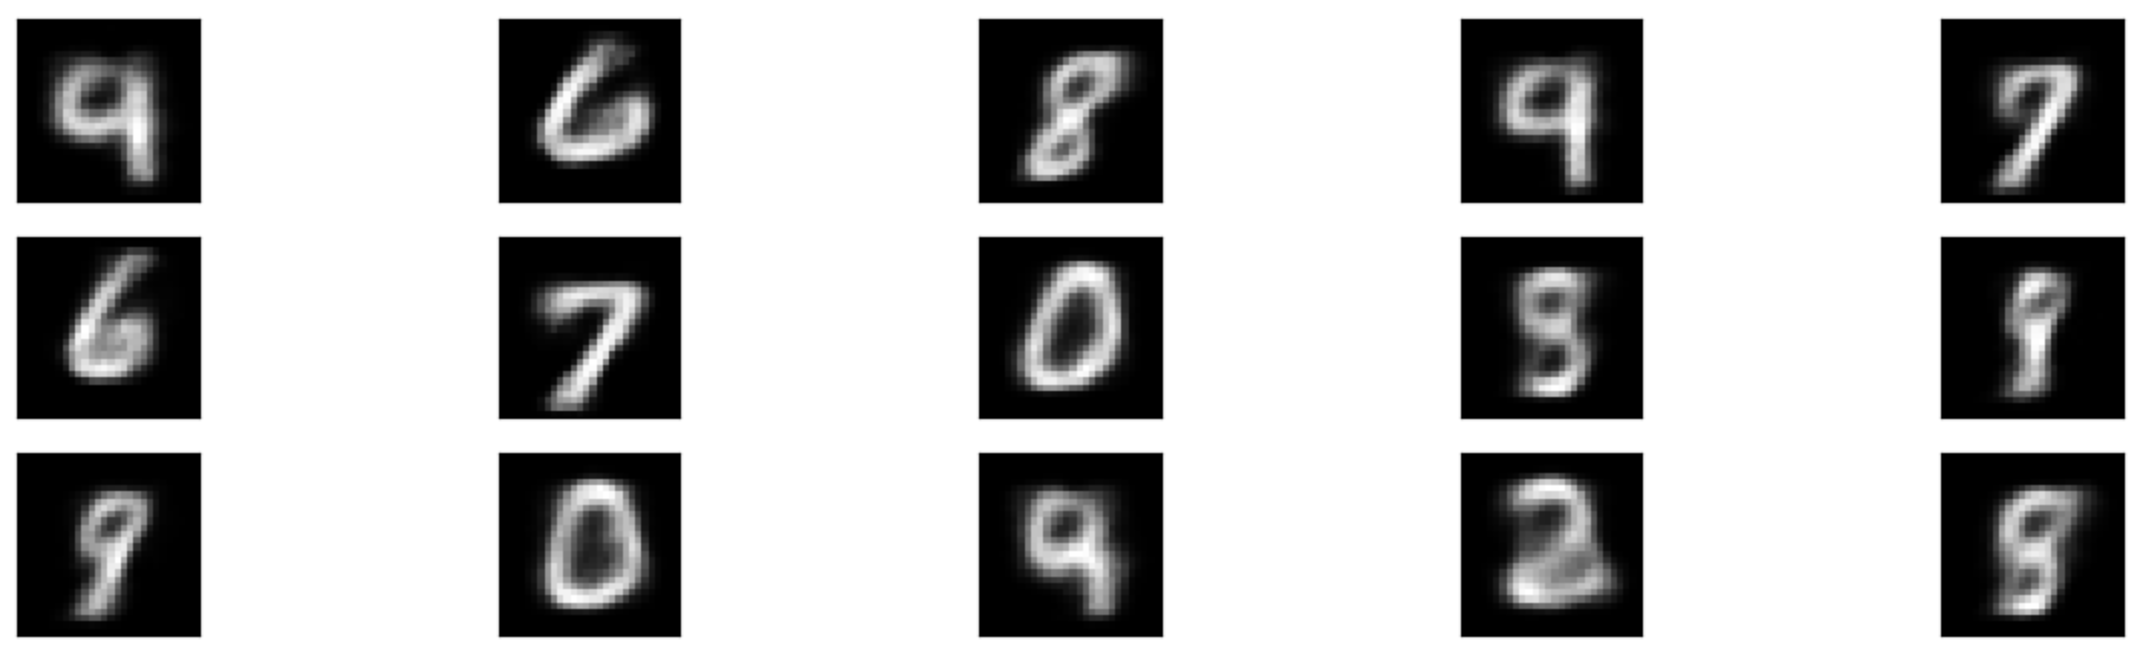
\includegraphics[width=\textwidth]{images/3-generated5.png}
        \caption{5 epochs}
        \label{fig:generated5}
    \end{subfigure}
    \begin{subfigure}[b]{\textwidth}
        \centering
        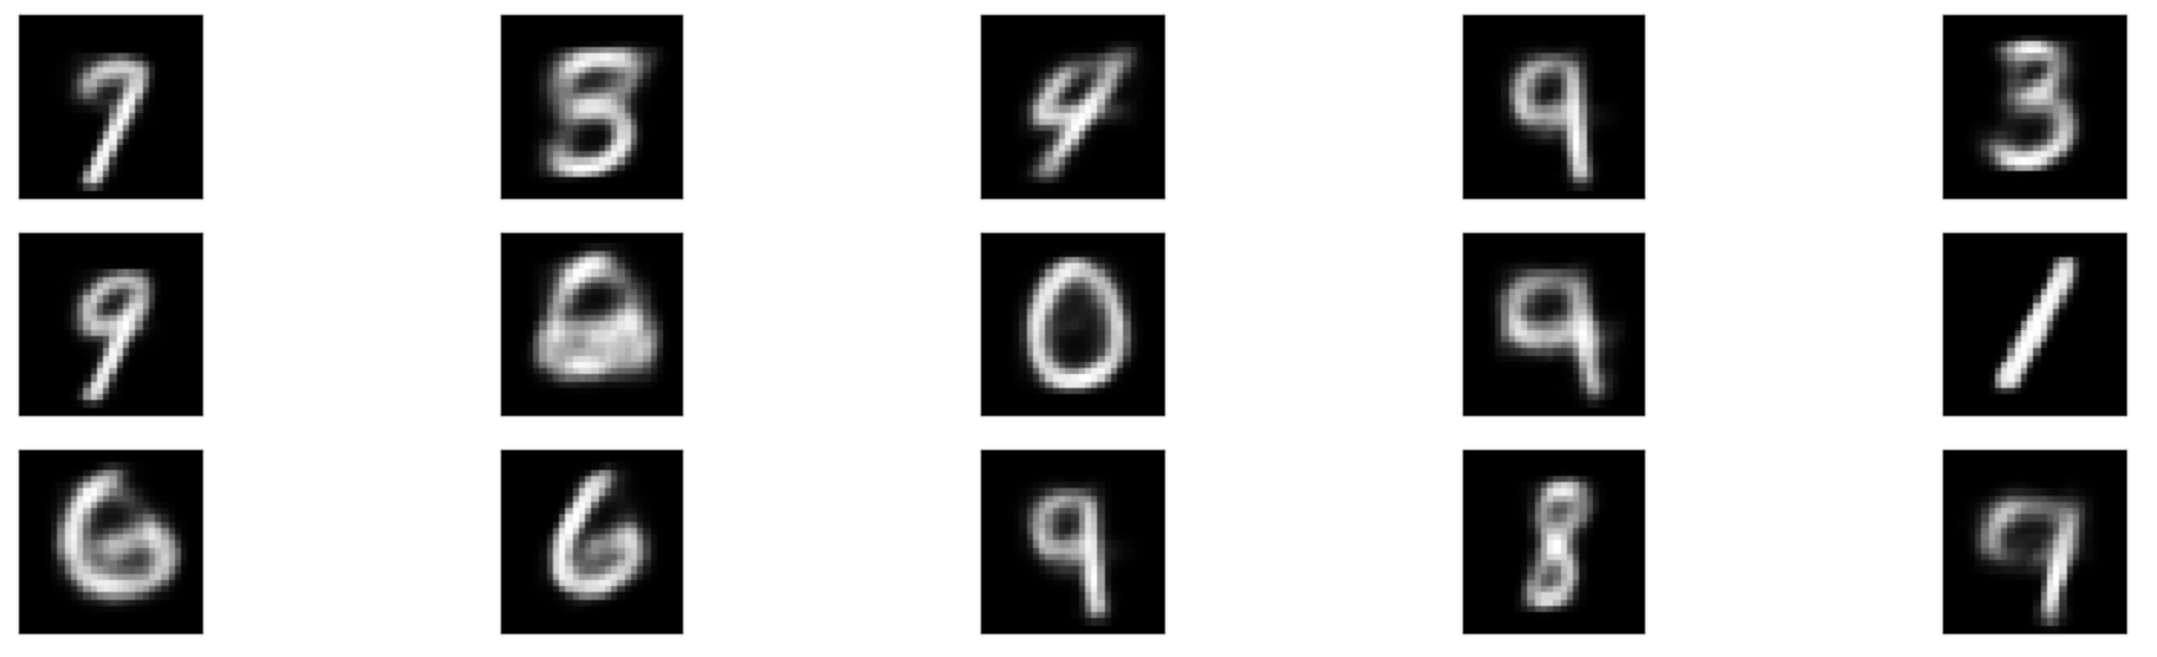
\includegraphics[width=\textwidth]{images/3-generated25.png}
        \caption{25 epochs}
        \label{fig:generated25}
    \end{subfigure}
    \begin{subfigure}[b]{\textwidth}
        \centering
        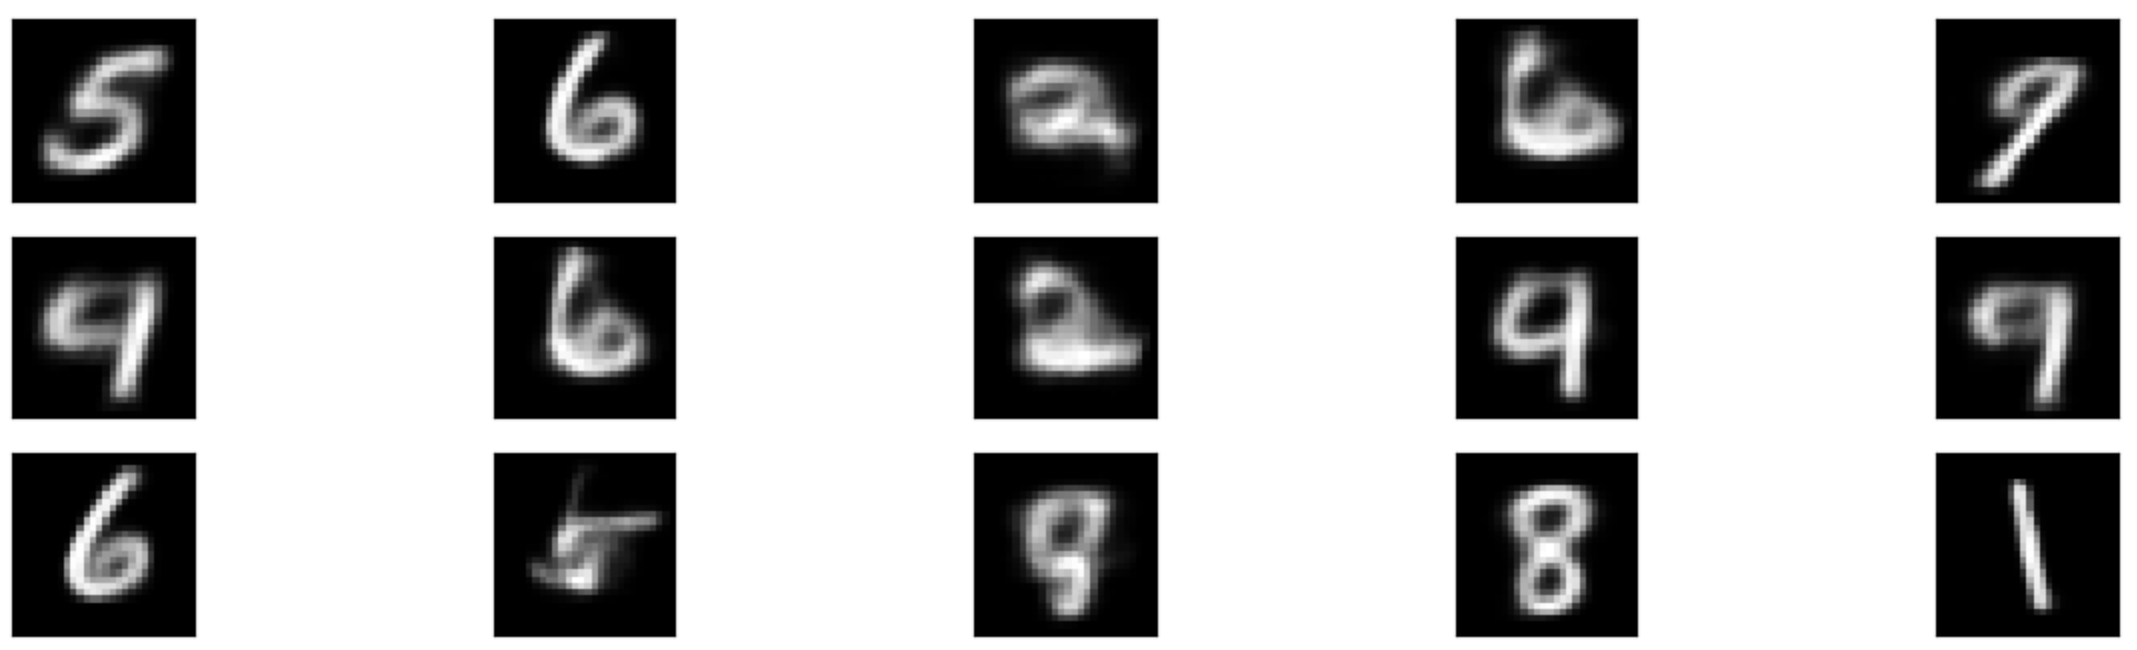
\includegraphics[width=\textwidth]{images/3-generated50.png}
        \caption{50 epochs}
        \label{fig:generated50}
    \end{subfigure}
    % generated after optimisation converged
    \caption{Generated digits after different numbers of epochs}
    \label{fig:generated}
\end{figure}

\begin{figure}[H]\ContinuedFloat
    \centering
    \begin{subfigure}[b]{\textwidth}
        \centering
        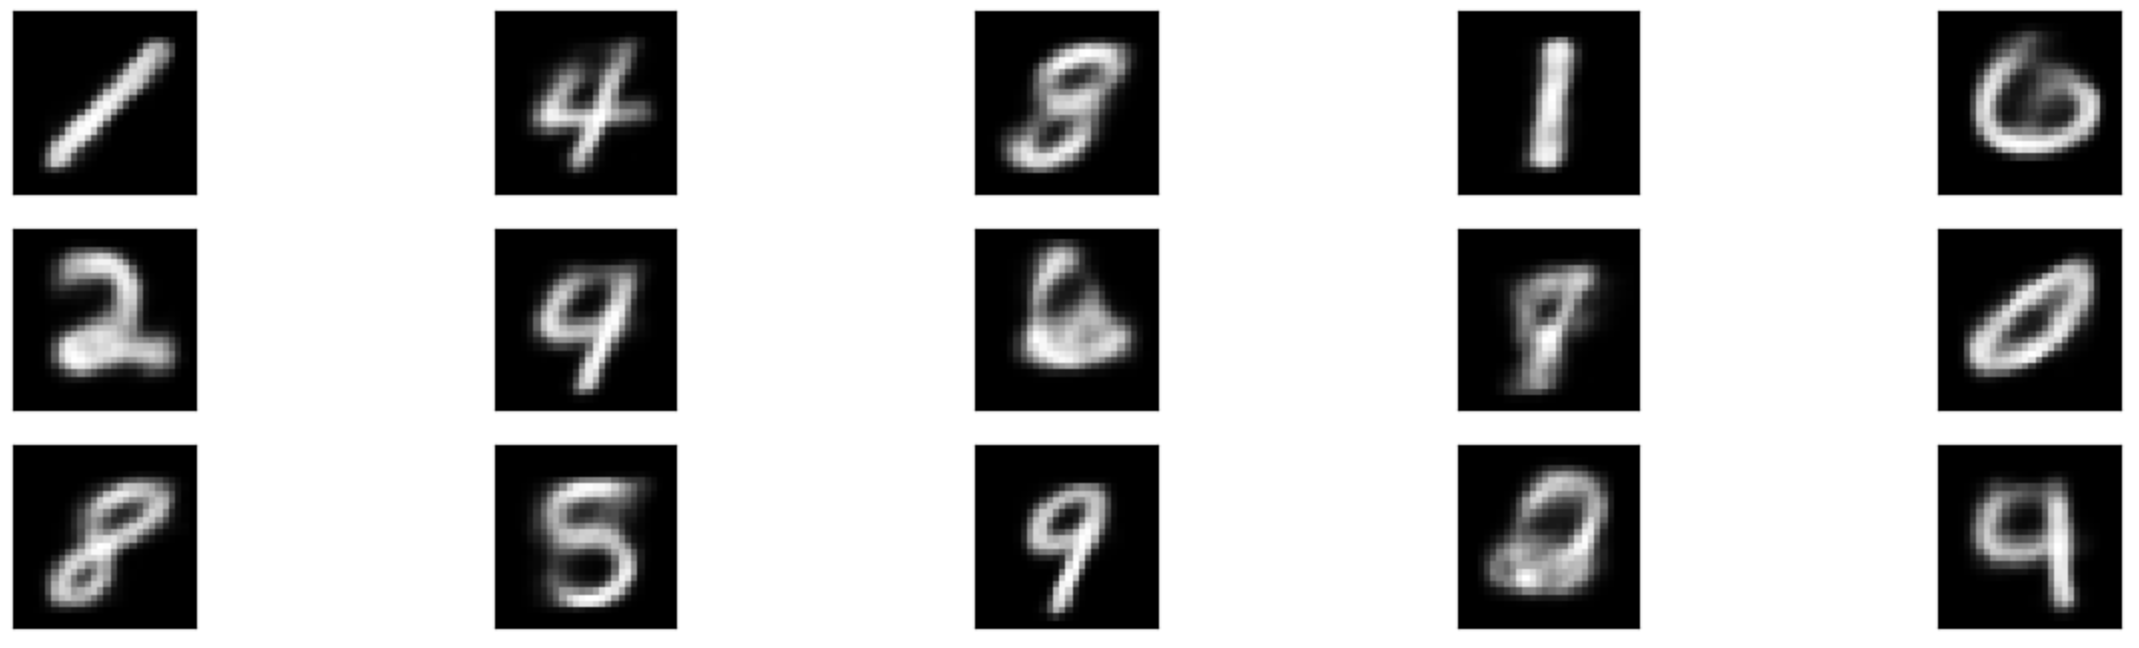
\includegraphics[width=\textwidth]{images/3-generatedCon.png}
        \caption{after convergence}
        \label{fig:generatedCon}
    \end{subfigure}
    \caption{Generated digits after different numbers of epochs}
    \label{fig:generated2}
\end{figure}

\textbf{4. Plot the loss curve} \\

ELBO loss stands for 'evidence lower bound loss' and is commonly used in VAEs. Figure \ref{fig:elbo} shows the loss development over the epochs. In the first two epochs, the training loss drops quickly to a value of $165.5712$, the test loss being slightly lower at $162.4413$. After that, the loss decreases slowly until we achieve a training loss of $141.2879$ and a test loss of $141.8026$. This behavior is what was expected. The values of training and test loss leave a small generalization gap, meaning that our model is able to perform well on unseen data as well. Since the training loss curve is still going down when we stop training, the model is not overfitting and we could possibly increase the training time (amount of epochs) to achieve the best possible outcome given the same parameters. \\ 

\begin{figure}[hbt!]
    \centering
    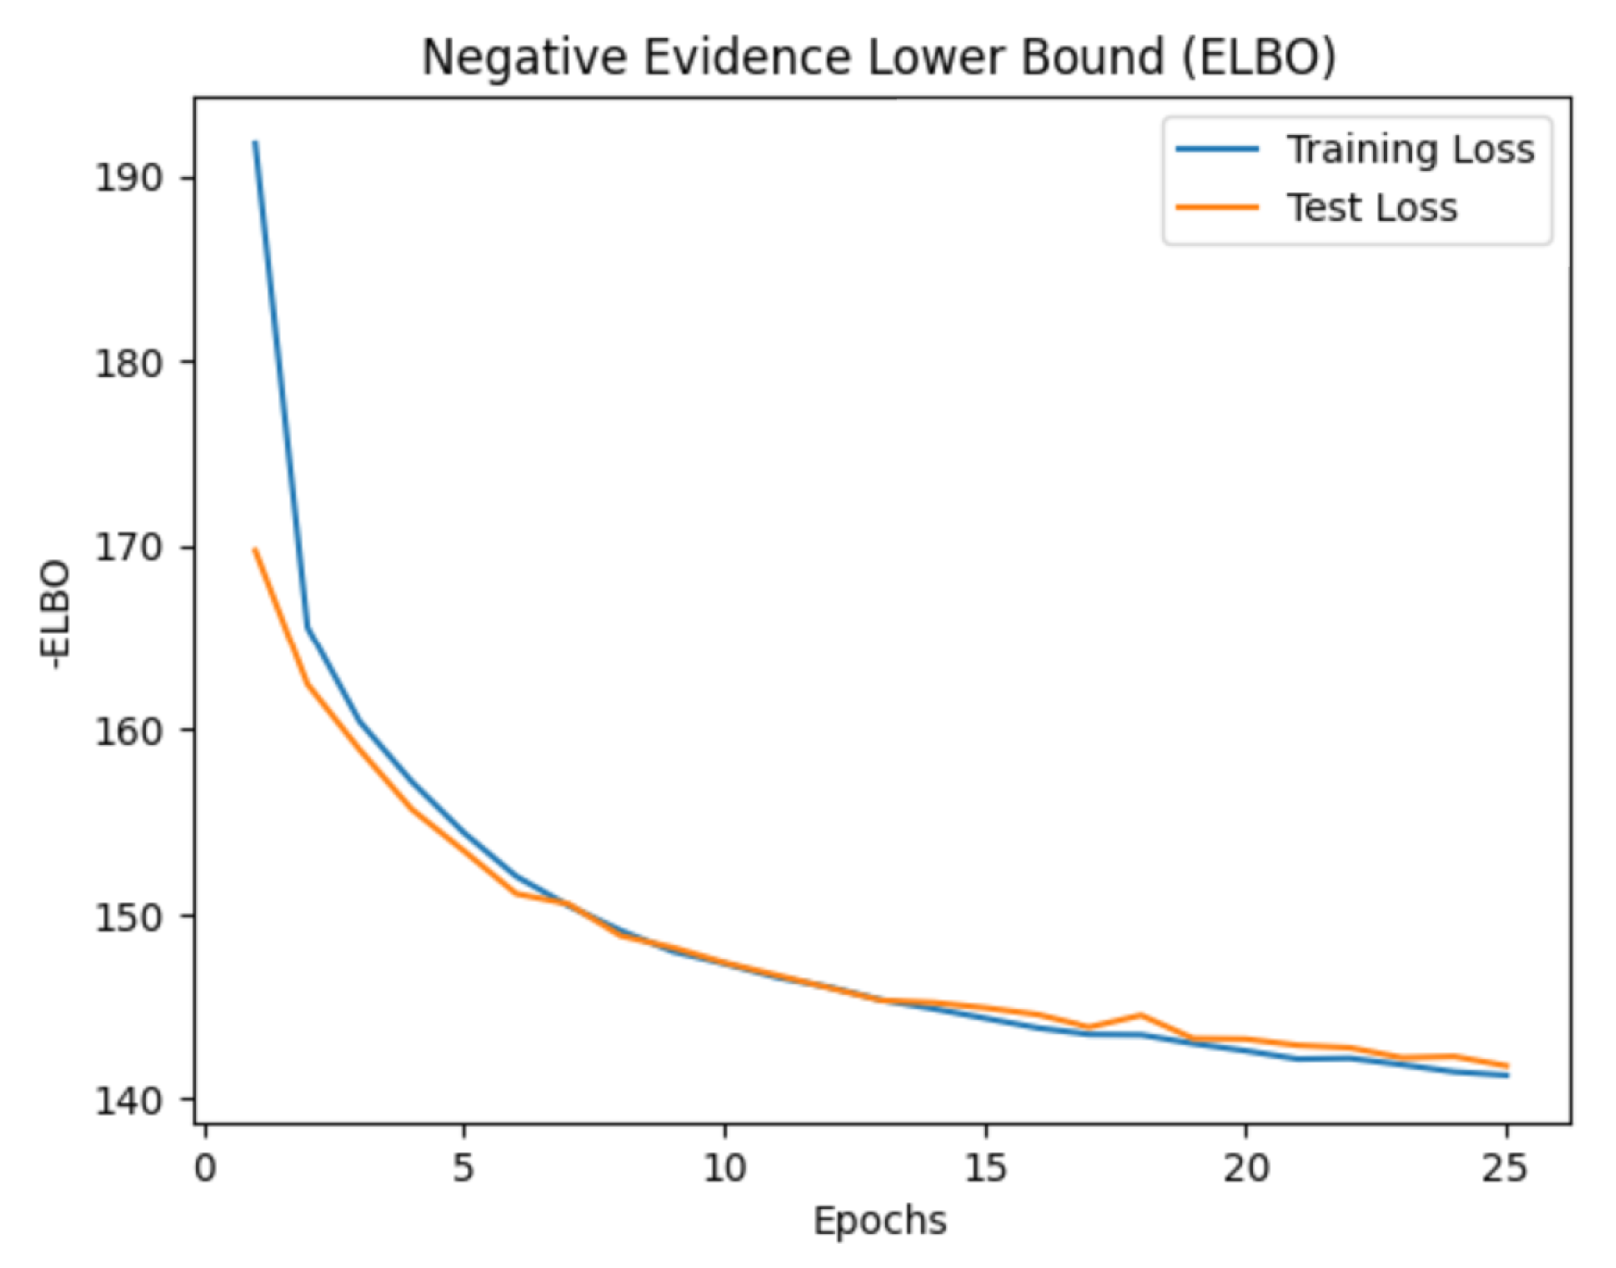
\includegraphics[width=0.7\textwidth]{images/3-ELBO.png}
    \caption{ELBO Loss vs. epochs on 2-dimensional latent space}
    \label{fig:elbo}
\end{figure}

\newpage
\textbf{5. Train the VAE using a 32-dimensional latent space} \\

% 5.1. Compare 15 generated digits with the results in 3.3.
Despite our assumption, increasing the latent space does not generate better digits with a training time of 25 epochs. In figure \ref{fig:generated-32}, the depicted digits are less recognizable, less than half of them can be assigned a certain number. \\


\begin{figure}[H]
    \centering
    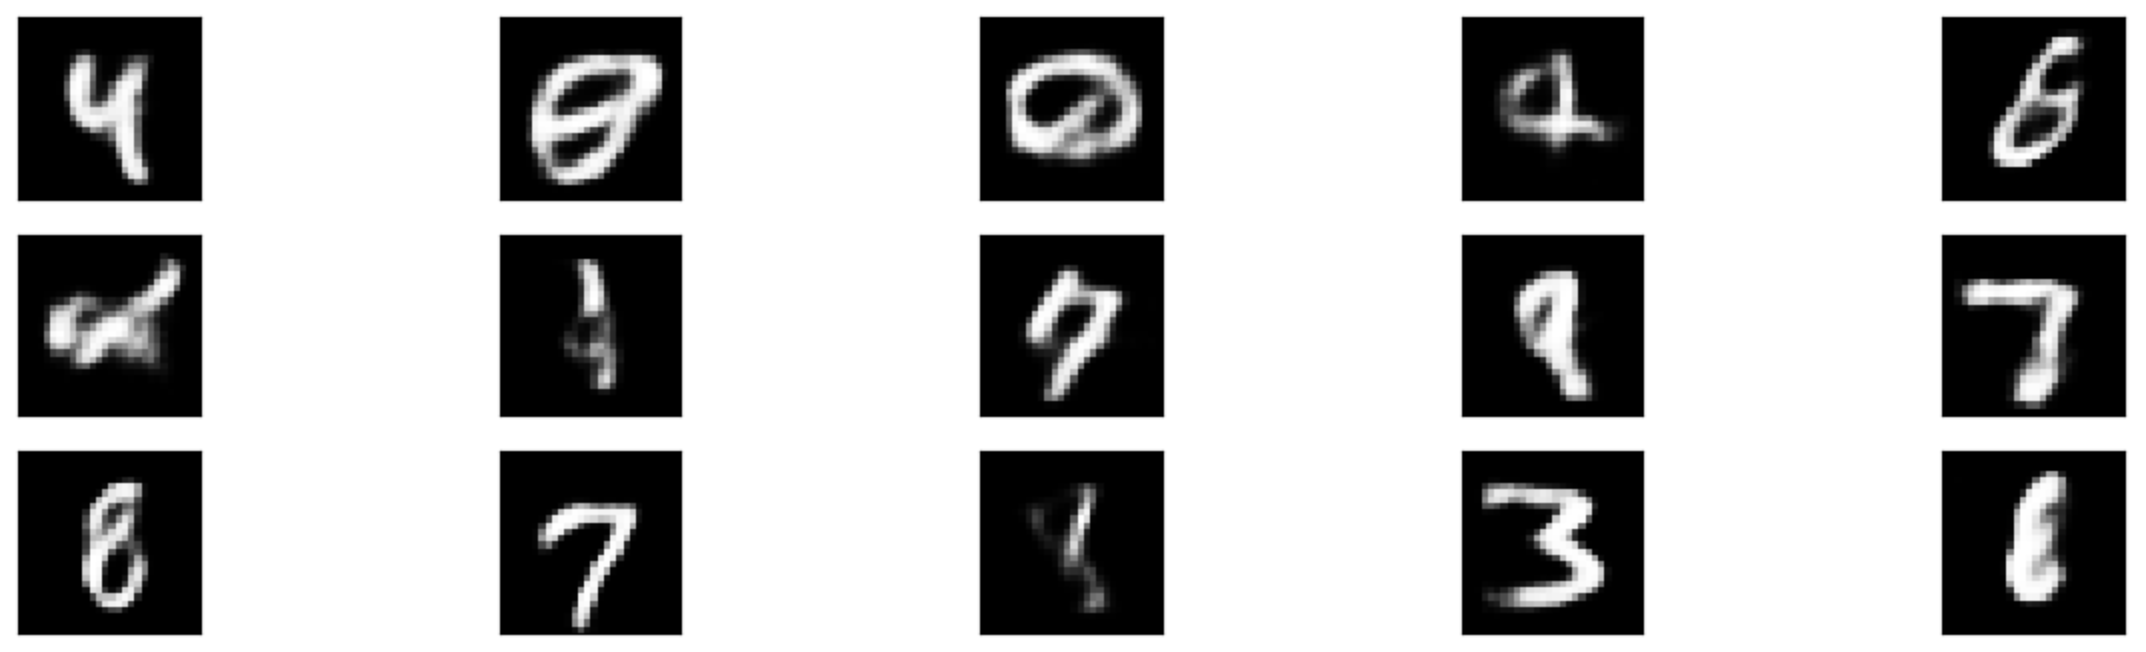
\includegraphics[width=\textwidth]{images/3-generated-32.png}
    \caption{Generated digits on 32-dimensional latent space}
    \label{fig:generated-32}
\end{figure}

% 5.2. Compare the loss curve with the one in 4.
At first glance, figure \ref{fig:elbo32} looks similar to the previously generated loss curve. Once we take a closer look, we notice that increasing the latent space to 32 has a positive effect on the loss: After just two epochs, the loss already dropped to $129.1468$ for the training and $120.9672$ for the test, both values are lower than the previous loss after our full training time. In comparison to the last test loss, it is more stable now and does not depict any spikes in its curve. After the 25th epoch, we reach a training loss of $101.1582$ and a test loss of $101.0482$ which is significantly better with a difference of roughly $40$ each. Again, we can see that the training loss is still decreasing in the end. This time, however, the decrease involves only decimals.  

\begin{figure}[H]
    \centering
    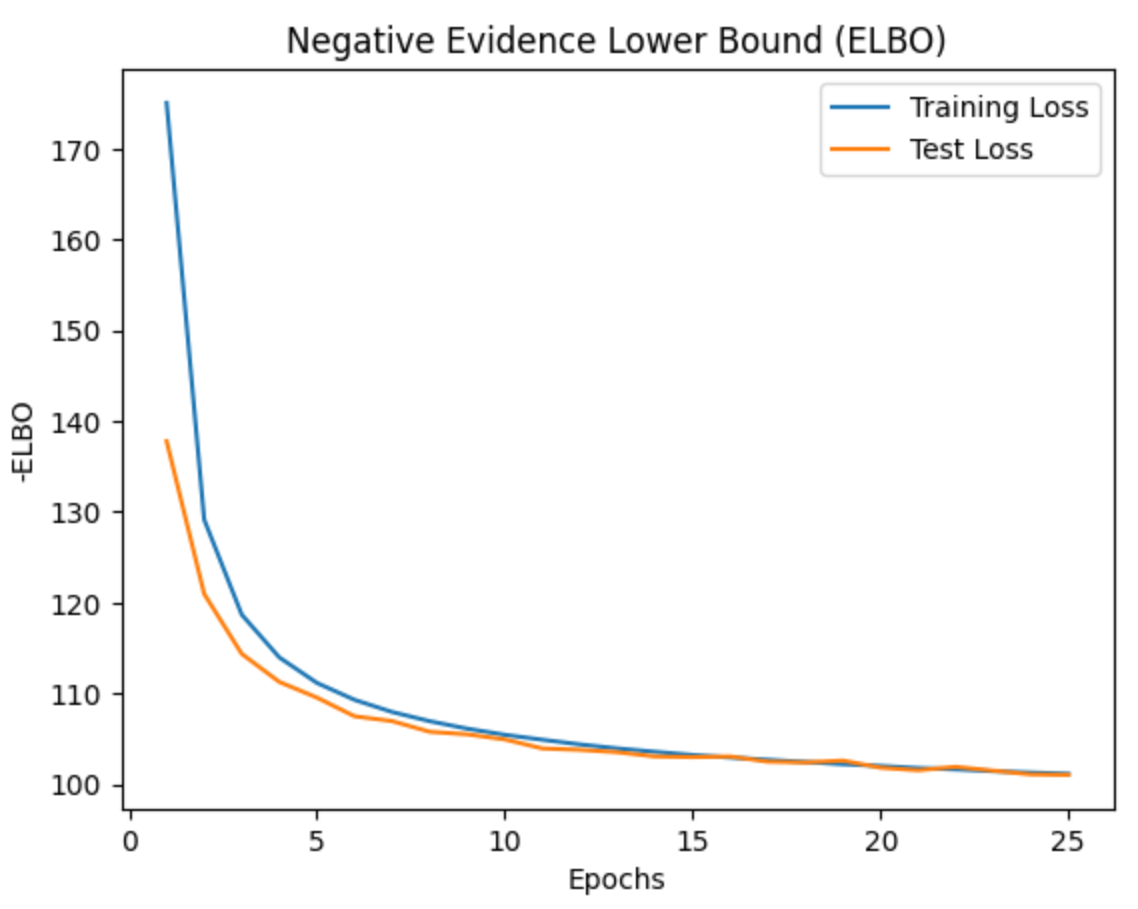
\includegraphics[width=0.7\textwidth]{images/3-ELBO32.png}
    \caption{ELBO Loss vs. epochs on 32-dimensional latent space}
    \label{fig:elbo32}
\end{figure}

% time estimate : 
Approximately 15hours have been needed in order to implement and test the VAE model itself.
% accuracy : 


% what we learned about data and method : 
    % by increasing the dimensionality of the latent space 
The observations made in 5. prove that simply increasing the latent space of a model doesn't necessarily improve its performance and it can be explained by the fact that the model isn't complex enough to deal with the added capacity of representation brought by the larger latent space and/or by the fact that the dataset's complexity (here the MNIST) doesn't warrant a larger latent space as it has a low intrinsic dimensionality itself. 